\chapter{Implementation and Experiment}

\section{Introduction}

\hspace{1cm} In the previous chapter, we introduced TOCL+, an extension of OCL with temporal operators and event constructs, and presented a theoretical framework for specifying and verifying temporal properties in UML models. While the formal semantics and verification approach provide a solid foundation, they require practical tool support to be effectively applied. This chapter bridges the gap between theory and practice by presenting our implementation of a TOCL+ plugin for the USE tool and demonstrating its effectiveness through a detailed case study.

The primary objective of this chapter is twofold. First, we describe the implementation of our TOCL+ plugin for the USE tool, which enables modelers to specify temporal properties using our extended language and automatically verify them using the filmstrip approach. Second, we demonstrate the practical application of TOCL+ through a detailed case study of the Software System model introduced in Chapter 2, showcasing how various types of temporal properties can be effectively specified and verified.

In the following sections, we present the architecture and implementation of our plugin, focusing on how it integrates with the USE tool environment and implements the transformation process described in Chapter 2. We then explore the Software System case study, illustrating how our approach handles the specification and verification of different types of temporal properties in practice.
\section{TOCL+ Tool Support and Implementation}

\subsection{Support tool architecture}

\begin{figure}
    \centering
    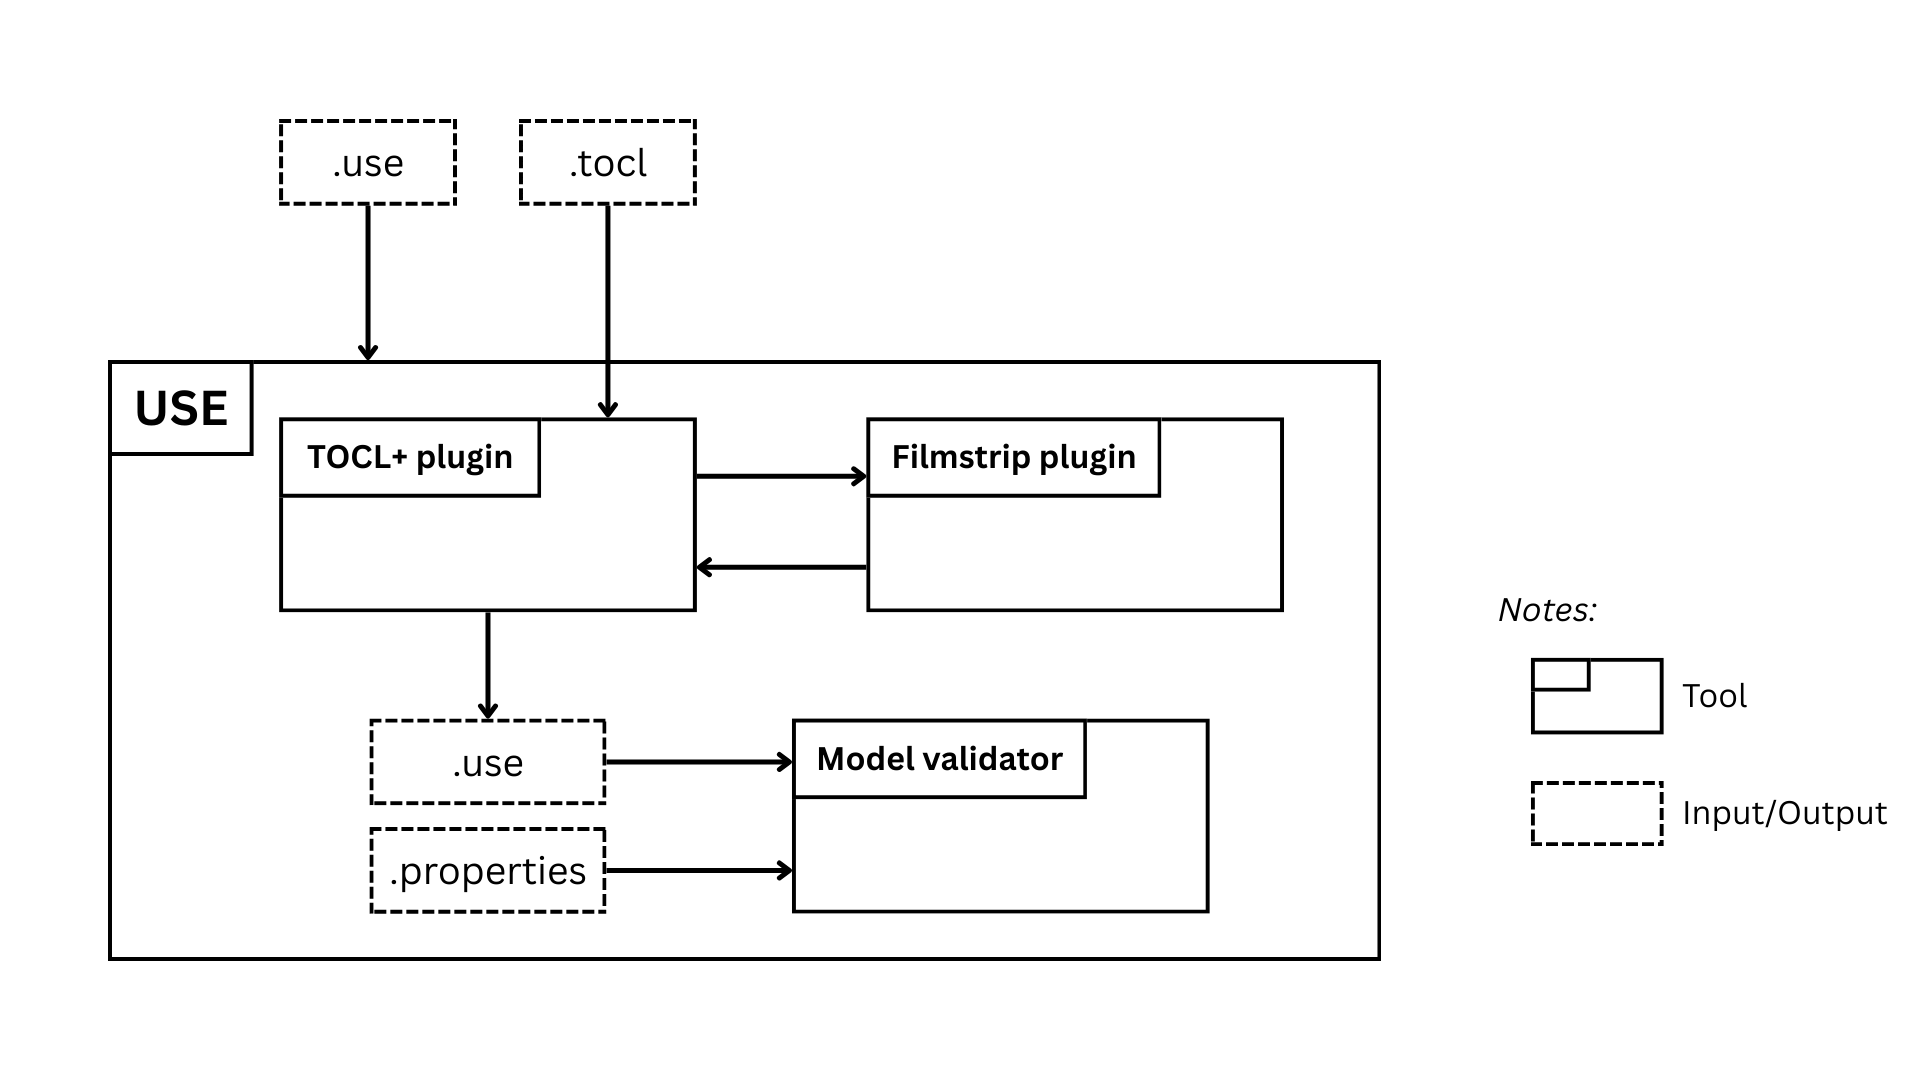
\includegraphics[width=1\textwidth]{figures/c3/Architecture_overview.png}
    \caption{Support Tool Architecture and Verification Workflow.}
    \label{sec:plugin_support_tool_architecture}
\end{figure}

\hspace{1cm} Figure \ref{sec:plugin_support_tool_architecture} illustrates the 
architecture and workflow of our TOCL+ support tool. This integrated verification 
framework combines several components: the existing USE environment, the Filmstrip 
plugin, our TOCL+ plugin, and the Model Validator. The architecture maintains a 
clear separation between modeling, specification, and verification concerns while 
providing a cohesive workflow for users.

The verification process consists of five distinct steps, beginning with preparation 
and ending with validation. First, the user prepares two input files: a standard 
\texttt{.use} file containing the UML/OCL application model and a \texttt{.tocl} 
file containing TOCL+ property specifications. Second, the user loads the application 
model into USE to make it available for transformation. Third, the user activates 
our plugin through the USE interface, selecting both a destination path for the 
output model and the \texttt{.tocl} file containing the temporal properties to verify.

Internally, the plugin then executes a two-phase transformation process. In the 
first phase, it invokes the Filmstrip plugin to transform the application model 
into a filmstrip model following the rules described in Section~\ref{subsec:filmstripping}. 
In the second phase, it processes the TOCL+ expressions using our ANTLR4-generated 
parser and listener components, which implement the transformation rules for 
converting temporal specifications into equivalent OCL constraints. These generated 
constraints are added to the list of invariants in the output model file alongside 
the filmstrip model elements.

To complete the verification process, the user loads this output model back into 
USE together with a configuration file that establishes search bounds, and then 
employs the Model Validator to analyze the constraints. The validator systematically 
explores the search space, determining whether the temporal properties are satisfied 
and providing a model instance as evidence when applicable.

Our primary contribution in this architecture is the TOCL+ plugin, specifically 
the TOCL+ to OCL transformation component that enables the verification of temporal 
properties using existing OCL tools. The implementation details of this transformation 
process, including the translation rules for different temporal operators and event 
constructs, are presented in the next subsection.

\subsection{Implementation of TOCL+ to OCL Transformation}

\hspace{1cm} The core of our contribution lies in the transformation of TOCL+ 
expressions into equivalent OCL constraints that can be verified over filmstrip 
models. This transformation process involves systematically mapping temporal operators 
and event constructs to structural navigations through snapshots and operation calls. 
In this section, we describe our implementation approach and the key translation 
patterns we developed.

Our transformation approach is inspired by the work of \cite{TOCL2OCL}, who 
transformed TOCL \cite{TOCL} into OCL in the context of a Snapshot-Transition Model 
(STM). While their approach also converts temporal properties into static ones, we 
adapted and extended it to work within the filmstrip model context.

To transform TOCL+ expressions, we defined translations for TOCL+ operators and 
events to OCL, as shown in Table \ref{tab:TOCL2OCL}. To create these translations, 
we utilized several query operations provided by the filmstrip structure. 
The self.snapshot query accesses the snapshot associated with an object in the 
"current state" where the expression is being evaluated. The pred() and succ() 
operations, when applied to a snapshot, navigate to the previous and next state 
respectively. For objects to navigate to their corresponding versions in adjacent 
states, we use the two associations .pred and .succ. These navigation mechanisms 
form the foundation for implementing our temporal operator translations.

Note that filmstrip model does not inherently provide any means to identify the same 
logical object across different states - it only provides the .pred and .succ 
associations to navigate between corresponding objects in adjacent snapshots. 
In order to overcome this limitation, we require modelers to add an id attribute 
to all classes in the application model. As seen in Figure \ref{fig:object_diagram_liveness}, 
this allows us to identify the same logical object across different snapshots. 
Internally, when the TOCL+ plugin transforms the model, we add additional 
constraints to ensure this id remains consistent between different states. 
This id attribute is critical in the OCL translation, particularly for event 
constructs like becomesTrue. When navigating with expressions like 
self.snapshot.pred().[ContextObject], we get a collection of objects of the same 
type, and we select the one with matching identity using ->any(o | o.id = self.id).

Table \ref{tab:TOCL2OCL} presents the complete set of translation patterns we 
developed for TOCL+ operators and event constructs. Each pattern systematically 
maps a TOCL+ construct to an equivalent OCL expression interpreted over the filmstrip 
model. The patterns use placeholders (indicated by square brackets) that get 
substituted during the transformation process: \texttt{[s |= P]} indicates that 
property P holds in snapshot s; \texttt{[ContextSnapshot]} is the snapshot in which 
the property is evaluated; \texttt{[ContextObject]} is the object on which the 
property is evaluated; and \texttt{[OpClassName]} is the class representing an 
operation call in the filmstrip model. When applying these patterns, each placeholder 
is replaced with the appropriate expression based on the model context. For example, 
in the liveness property translation shown in Listing \ref{lst:ocl_liveness}, the 
\texttt{[ContextSnapshot]} is replaced with the local variable \texttt{s} inside the 
\texttt{exists} query. The bounded quantifiers (e.g., \texttt{at most}, \texttt{at least}) 
are translated into corresponding comparators (\texttt{<=}, \texttt{>=}). 
The bounded quantifiers in TOCL+ expressions are systematically translated into their 
corresponding OCL comparators: \texttt{at most} becomes less than or equal to 
(\texttt{<=}), while \texttt{at least} becomes greater than or equal to (\texttt{>=}). 
For bounded existence properties without an explicit quantifier (e.g., 
\texttt{isCalled(Op()) 3 times}), the translation applies the equality operator 
(\texttt{=}), enforcing that the event occurs exactly the specified number of times. 
In contrast, when dealing with unbounded event expressions without quantifiers (e.g., 
simply \texttt{isCalled(Op())}), the translation converts the \texttt{select} operation 
into an \texttt{exists} operation, requiring only that the event occurs at least once 
rather than counting occurrences.
    
We implemented the transformation using ANTLR4, a parser generator that creates a 
parse tree from TOCL+ expressions. After defining the translation patterns shown 
in Table \ref{tab:TOCL2OCL}, we created Java listener classes that extend the 
generated parser listeners. The transformation process employs these listener 
components to traverse the parse tree and produce corresponding OCL expressions 
by overriding the generated listener methods. As the parser walks through each node 
in the parse tree, our listeners intercept parse tree events and apply the appropriate 
translation rules, constructing equivalent OCL constraints that navigate through 
the filmstrip structure. The transformation follows a consistent pattern: when a 
temporal operator or event construct is encountered, the listener extracts relevant 
information from the parse tree nodes, applies the corresponding translation pattern, 
and builds the equivalent OCL expression. Our implementation maintains a stack of 
expressions to handle nested structures, pushing both the original TOCL+ expression 
and its OCL translation for later integration into the output model.
Listing \ref{lst:becomesTrue_translation} provides an example of this process for 
the \texttt{becomesTrue} event construct, showing how we extract the expression 
to be evaluated, establish the necessary context, and construct the translated OCL 
expression. 

After processing all the nodes in the parse tree, our implementation finalizes the 
translation in the root node visit. Since TOCL+ is an extension of OCL, many 
constructs remain unchanged and are directly preserved during translation. The 
completion process begins by accessing the token stream to retrieve the complete 
original expression text. Our implementation then systematically pops each translated 
OCL fragment and its corresponding original TOCL+ expression from the stack. Using 
string replacement operations, it substitutes each temporal construct with its 
equivalent OCL translation while preserving the structure of the original expression. 
This approach allows us to handle nested temporal operators naturally, as inner 
expressions are processed before their containing expressions. The final translated 
OCL constraint is then attached to the root of the parse tree and ultimately added 
to the output model as an invariant. This complete process ensures that complex 
temporal properties are accurately transformed into standard OCL constraints that 
can be verified by the Model Validator.

\begin{lstlisting}[
    style=javastyle,
    caption={Translation of becomesTrue event to OCL.},
    label={lst:becomesTrue_translation}
]
TokenStream tokens = parser.getTokenStream();
String originalEvent = tokens.getText(ctx);
String translatedEvent;
// P
String expressionToSatisfy = getOCL(ctx.getChild(2)); 
// e.g., "system", "application"
String roleName = toLowerFirstChar(currentContext); 
String currentSnapshot = "self.snapshot"; 
String selectObject = "->any(o | o.id = self.id)";

// e.g. self.snapshot.system->any(o | o.id = self.id)
String objectAtCurrentSnapshot = currentSnapshot + "." + roleName + selectObject;
String objectAtPreviousSnapshot = currentSnapshot + ".pred()." + roleName + selectObject;
String P_at_currentSnapshot = expressionToSatisfy.replace("self", "currentObject");
String P_at_previousSnapshot = expressionToSatisfy.replace("self", "previousObject");

translatedEvent = 
"let currentObject = " + objectAtCurrentSnapshot +
" in let previousObject = " + objectAtPreviousSnapshot +
" in not (" + P_at_previousSnapshot + ") and (" + P_at_currentSnapshot + ")";

eventStack.push(translatedEvent);
eventStack.push(originalEvent);    
\end{lstlisting}

\begin{longtable}{|>{\footnotesize}p{0.6cm}|>{\scriptsize\raggedright\arraybackslash}p{4cm}|>{\scriptsize\raggedright\arraybackslash}p{\dimexpr\textwidth-4.6cm-4\tabcolsep-3\arrayrulewidth\relax}|}
    \caption{Translation of TOCL+ operators and events to OCL.}
    \label{tab:TOCL2OCL} \\
    \hline
    \textbf{No.} & \textbf{TOCL+} & \textbf{OCL Translation} \\
    \hline
    1 & 
    next P &
    let nextSnapshot:Snapshot = self.snapshot.succ() in [nextSnapshot |= P] \\
    \hline
    2 &
    always P &
    let CS:Snapshot = self.snapshot in Set\{CS\}->closure(s | s.succ())->forAll(s | [s |= P]) \\
    \hline  
    3 &
    always P until Q &
    let CS:Snapshot = self.snapshot
    in let FS:Set(Snapshot) = Set\{CS.succ()\}->closure(s | s.succ())
    in let AllFSQ:Set(Snapshot) = FS->select(s | [s |= Q])
    in let FSQ:Snapshot = AllFSQ->any(s | Set\{s\}->closure(s | s.succ())->includesAll(AllFSQ))
    in let afterQ:Set(Snapshot) = Set\{FSQ\}->closure(s | s.succ())
    in let FSP:Set(Snapshot) = FS->select(s | [s |= P])
    in if FSQ.isDefined() then (if (FSP->size() > 0) then (FS-afterQ = FSP-afterQ) else false endif) else (FS = FSP) endif \\
    \hline
    4 &
    always P since Q &
    let CS:Snapshot = self.snapshot
    in let PS:Set(Snapshot) = Set\{CS.pred()\}->closure(s | s.pred())
    in let AllPSQ:Set(Snapshot) = PS->select(s | [s |= Q])
    in let PSQ:Snapshot = AllPSQ->any(s | Set\{s\}->closure(s | s.pred())->includesAll(AllPSQ))
    in let beforeQ:Set(Snapshot) = Set\{PSQ\}->closure(s | s.pred())
    in let PSP:Set(Snapshot) = PS->including(CS)->select(s | [s |= P])
    in if PSQ.isDefined() then (if (PSP->size() > 0) then (PS->including(CS)-beforeQ = PSP-beforeQ) else false endif) else (PSP = PS->including(CS)) endif \\
    \hline
    5 &
    sometime P &
    let CS:Snapshot = self.snapshot in Set\{CS\}->closure(s | s.succ())->exists(s | [s |= P]) \\
    \hline
    6 &
    sometime P before Q &
    let FS:Set(Snapshot) = Set\{self.snapshot\}->closure(s | s.succ())
    in let PreS:Set(Snapshot) = Set\{self.snapshot.pred()\}->closure(s | s.pred())
    in let AllFSQ:Set(Snapshot) = FS->select(s | [s |= Q])
    in let FSQ:Snapshot = AllFSQ->any(s | Set\{s\}->closure(s | s.succ())->includesAll(AllFSQ))
    in let FSP:Set(Snapshot) = FS->select(s | [s |= P])
    in if FSQ.isDefined() then (if (FSP->size() > 0) then ((Set\{FSQ.pred()\}->closure(s | s.pred())-PreS)->exists(s\_1 | FSP->includes(s\_1))) else false endif) else false endif \\
    \hline
    7 &
    sometime P since Q &
    let CS:Snapshot = self.snapshot
    in let PS:Set(Snapshot) = Set\{CS.pred()\}->closure(s | s.pred())
    in let AllPSQ:Set(Snapshot) = PS->select(s | [s |= Q])
    in let PSQ:Snapshot = AllPSQ->any(s | Set\{s\}->closure(s | s.pred())->includesAll(AllPSQ))
    in let PSP:Set(Snapshot) = PS->select(s | [s |= P])
    in if PSQ.isDefined() then (Set{PSQ}->closure(s | s.succ())->excluding(null)->intersection(PS)->exists(s | PSP->includes(s))) else false endif \\ 
    \hline
    8 &
    previous P &
    let previousSnapshot:Snapshot = self.snapshot.pred() in [previousSnapshot |= P] \\
    \hline
    9 &
    sometimePast P &
    let CS:Snapshot = self.snapshot in Set\{CS.pred()\}->closure(s | s.pred())->exists(s | [s |= P]) \\
    \hline
    10 &
    alwaysPast P &
    let CS:Snapshot = self.snapshot in Set\{CS.pred()\}->closure(s | s.pred())->forAll(s | [s |= P]) \\
    \hline
    11 &
    isCalled(Op()) &
    [OpClassName].allInstances()->exists(op | op.succ() = [ContextSnapshot]) \\
    \hline
    12 &
    isCalled(Op($param_1$, $\ldots$, $param_n$)) &
    [OpClassName].allInstances()->exists(op | op.succ() = [ContextSnapshot] and
    (Set\{op.$param_1$.succ\}->closure(p | p.succ)->includes($param_1$) or Set\{op.$param_1$.pred\}->closure(p | p.pred)->includes($param_1$))
    and ($\ldots$)
    and (Set\{op.$param_n$.succ\}->closure(p | p.succ)->includes($param_n$) or Set\{op.$param_n$.pred\}->closure(p | p.pred)->includes($param_n$))) \\
    \hline
    13 &
    isCalled(Op()) [at most | at least | ] n times &
    [OpClassName].allInstances()->select(op | op.succ() = [ContextSnapshot])->size() [<= | >= | =] n \\
    \hline
    14 &
    isCalled(Op($param_1$, $\ldots$, $param_n$)) [at most | at least | ] n times &
    [OpClassName].allInstances()->select(op | op.succ() = [ContextSnapshot] and
    (Set\{op.$param_1$.succ\}->closure(p | p.succ)->includes($param_1$) or Set\{op.$param_1$.pred\}->closure(p | p.pred)->includes($param_1$)) 
    and ($\ldots$) 
    and (Set\{op.$param_n$.succ\}->closure(p | p.succ)->includes($param_n$) or Set\{op.$param_n$.pred\}->closure(p | p.pred)->includes($param_n$)))->size() [<= | >= | =] n \\
    \hline
    15 &
    becomesTrue(P) &
    let currentObject = self.snapshot.[ContextObject]->any(o | o.id = self.id) in
    let previousObject = self.snapshot.pred().[ContextObject]->any(o | o.id = self.id) in 
    not [previousObject |= P] and [currentObject |= P] \\
    \hline
\end{longtable}

\section{Case study: Software System model}
\label{sec:case_study_software_system}

\subsection{Model Specification}

The Software System model shown in Listing \ref{lst:software_system_specification} 
is the same model introduced in Chapter 1 to demonstrate OCL constraints (see 
Figure \ref{fig:class_diagram_software_system}). As a reminder, this model represents 
a simplified operating system that manages applications through their lifecycle. 
It consists of two main classes: \texttt{System} and \texttt{Application}, connected 
through an association. The \texttt{System} maintains three collections 
(\texttt{loadedApps}, \texttt{installedApps}, and \texttt{runningApps}) representing 
different application states, and provides four operations to manage applications: 
\texttt{load}, \texttt{install}, \texttt{run}, and \texttt{stop}.

The \texttt{freeMemory} attribute represents available disk space, which decreases 
when applications are loaded. The \texttt{load} operation acts as a download action, 
reducing available memory when an application is acquired. The \texttt{install} 
operation processes all loaded applications at once, moving them from 
\texttt{loadedApps} to \texttt{installedApps}. When an application is running, it 
exists in both the \texttt{installedApps} and \texttt{runningApps} sets simultaneously. 
The \texttt{SystemApplication} association facilitates navigation between system and 
applications in this simplified model.

Note that the numerous postconditions like \texttt{sameInstalledAndRunning}, 
\texttt{sameRunning}, \texttt{sameMemory}, \texttt{sameLoaded}, \texttt{sameInstalled}, 
and the \texttt{unchanged} constraints serve as helper constraints in the verification 
context: since the Model Validator assigns random values to attributes when exploring 
possible states, these constraints ensure that attributes unaffected by an operation 
remain consistent between snapshots.

This model serves as an ideal case study for temporal property verification as it 
involves operations with clear sequential dependencies and state transitions that 
cannot be adequately expressed using standard OCL. The full specification below 
includes all constraints and operation contracts necessary for our verification 
experiments.

\begin{lstlisting}[
    caption={Specification of the Software System model in USE environment.},
    label={lst:software_system_specification}
]
model SoftwareSystem
-- Classes
class System
attributes
    id : Integer
    freeMemory : Integer init = 10
    loadedApps : Set(Application) init = Set{}
    installedApps : Set(Application) init = Set{}
    runningApps : Set(Application) init = Set{}
operations
    load(app : Application)
    begin
        self.loadedApps := self.loadedApps->including(app);
        self.freeMemory := self.freeMemory - app.size;
    end
    install()
    begin
        self.installedApps := self.installedApps->union(self.loadedApps);
        self.loadedApps := self.loadedApps->reject(true)->excluding(null);
    end
    run(app : Application)
    begin
        self.runningApps := self.runningApps->including(app);
    end
    stop(app : Application)
    begin
        self.runningApps := self.runningApps->excluding(app);
    end
end
class Application
attributes
    id : Integer
    size : Integer
end
-- Associations
association SystemApplication between
    System[1] role system
    Application[0..*] role apps
end
-- Invariants
constraints
context System
    inv memoryConstraint: self.freeMemory >= 0
    inv notLoadedAndInstalled: self.loadedApps->intersection(self.installedApps)->isEmpty()
    inv sets: let appNumber: Integer = self.apps->size() in
        (self.loadedApps->size() <= appNumber and
        self.installedApps->size() <= appNumber and
        self.runningApps->size() <= appNumber)
    inv notContainsNull:
        not self.loadedApps->includes(null) and
        not self.installedApps->includes(null) and
        not self.runningApps->includes(null)

context Application
    inv sizeConstraint: self.size > 0

context System::load(app: Application)
    pre notLoaded: not self.loadedApps->includes(app) and
                    not self.installedApps->includes(app) and
                    not self.runningApps->includes(app)
    pre enoughMemory: self.freeMemory >= app.size
    post loaded: self.loadedApps = self.loadedApps@pre->including(app)
    post freeMemory: self.freeMemory = self.freeMemory@pre - app.size
    post unchanged:
        self.apps->forAll(app |
            app.size = app.size@pre and
            app.id = app.id@pre)
    post sameInstalledAndRunning:
        self.installedApps = self.installedApps@pre and
        self.runningApps = self.runningApps@pre

context System::install()
    pre hasLoadedApps: self.loadedApps->notEmpty()
    post installed: self.installedApps = self.installedApps@pre->union(self.loadedApps@pre)
    post loadedAppsEmpty: self.loadedApps = self.loadedApps@pre->reject(true)->excluding(null)
    post sameRunning: self.runningApps = self.runningApps@pre
    post sameMemory: self.freeMemory = self.freeMemory@pre
    post unchanged:
        self.apps->forAll(app |
            app.size = app.size@pre and
            app.id = app.id@pre)

context System::run(app : Application)
    pre isInstalled: self.installedApps->includes(app)
    pre notRunning: not self.runningApps->includes(app)
    post running: self.runningApps = self.runningApps@pre->including(app)
    post sameLoaded: self.loadedApps = self.loadedApps@pre
    post sameInstalled: self.installedApps = self.installedApps@pre
    post sameMemory: self.freeMemory = self.freeMemory@pre
    post unchanged:
        self.apps->forAll(app |
            app.size = app.size@pre and
            app.id = app.id@pre)

context System::stop(app : Application)
    pre isRunning: self.runningApps->includes(app)
            and self.installedApps->includes(app)
    post notRunning: self.runningApps = self.runningApps@pre->excluding(app)
    post sameInstalled: self.installedApps = self.installedApps@pre
    post sameLoaded: self.loadedApps = self.loadedApps@pre
    post sameMemory: self.freeMemory = self.freeMemory@pre
    post unchanged:
        self.apps->forAll(app |
            app.size = app.size@pre and
            app.id = app.id@pre)
\end{lstlisting}


\subsection{Temporal Property Verification}
% For each of the 4 properties:
%   1. Brief description of what the property verifies
%   2. TOCL+ specification
%   3. Generated OCL translation
%   4. Verification results

% The TOCL+ temporal properties for the Software System model were shown in Listing 
% \ref{lst:tocl+}. And Listing \ref{lst:ocl_translations} shows the OCL translations 
% for those TOCL+ properties. 

To demonstrate our TOCL+ to OCL transformation approach, we verified four temporal 
properties from Chapter 2 against the Software System model: safety1 (applications 
must be loaded before being run), safety2 (applications must follow the 
load-install-run sequence), safety3 (applications are loaded at most once), and 
liveness (loaded applications will eventually be installed). Listing 
\ref{lst:ocl_translations} shows the OCL constraints generated by our transformation 
plugin for these properties. While the resulting OCL expressions are considerably 
more complex than their TOCL+ counterparts—involving extensive navigation through 
the filmstrip model—they correctly implement the required temporal semantics. This 
demonstrates how our approach enables temporal reasoning within standard OCL, 
shielding modelers from the underlying complexity.

\begin{lstlisting}[
    caption={OCL Translations for TOCL+ properties shown in listing \ref{lst:tocl+}.},
    label={lst:ocl_translations}
]
context System
inv safety1:
    self.runningApps->notEmpty() implies
    self.runningApps->forAll(app |
        (run_SystemOpC.allInstances()->exists(op | op.succ() = self.snapshotSystem and (Set{op.app.succApplication}->closure(p | p.succApplication)->includes(app) or Set{op.app.predApplication}->closure(p | p.predApplication)->includes(app)))) implies
        (let CS:Snapshot = self.snapshotSystem in Set{CS.pred()}->closure(s | s.pred())->exists(s | (load_SystemOpC.allInstances()->exists(op | op.succ() = s and (Set{op.app.succApplication}->closure(p | p.succApplication)->includes(app) or Set{op.app.predApplication}->closure(p | p.predApplication)->includes(app))))))
    )

context System
inv safety2:
    self.runningApps->notEmpty() implies
    self.runningApps->forAll(app |
        (run_SystemOpC.allInstances()->exists(op | op.succ() = self.snapshotSystem and (Set{op.app.succApplication}->closure(p | p.succApplication)->includes(app) or Set{op.app.predApplication}->closure(p | p.predApplication)->includes(app)))) implies
        (let CS:Snapshot = self.snapshotSystem in let PS:Set(Snapshot) = Set{CS.pred()}->closure(s | s.pred())->excluding(null) in let AllPSQ:Set(Snapshot) = PS->select(s | (load_SystemOpC.allInstances()->exists(op | op.succ() = s and (Set{op.app.succApplication}->closure(p | p.succApplication)->includes(app) or Set{op.app.predApplication}->closure(p | p.predApplication)->includes(app))))) in let PSQ:Snapshot = AllPSQ->any(s | Set{s}->closure(s | s.pred())->includesAll(AllPSQ)) in let PSP:Set(Snapshot) = PS->select(s | install_SystemOpC.allInstances()->exists(op | op.succ() = s)) in if PSQ.isDefined() then (Set{PSQ}->closure(s | s.succ())->excluding(null)->intersection(PS)->exists(s | PSP->includes(s))) else false endif)
    )

context System
inv safety3:
    self.installedApps->notEmpty() implies
    self.installedApps->forAll(app |
        (let CS:Snapshot = self.snapshotSystem in Set{CS.pred()}->closure(s | s.pred())->exists(s | (load_SystemOpC.allInstances()->select(op | op.succ() = s and (Set{op.app.succApplication}->closure(p | p.succApplication)->includes(app) or Set{op.app.predApplication}->closure(p | p.predApplication)->includes(app)))->size() <= 1)))
    )

context System
inv liveness:
    self.loadedApps->notEmpty() implies
    self.loadedApps->forAll(app |
        (let CS:Snapshot = self.snapshotSystem in Set{CS}->closure(s | s.succ())->excluding(null)->exists(s | install_SystemOpC.allInstances()->exists(op | op.succ() = s)))
    )
\end{lstlisting}


\subsection{Analysis of Results}
% Figure \ref{fig:object_diagram_case_study} shows a scenario generated by the USE Model
% Validator. The scenario represents a system execution path start with loading an 
% application, installing it, running it, and stopping it. The OCL result for this
% scenario is shown in Figure \ref{fig:ocl_result_case_study}. 

\hspace{1cm} Figure \ref{fig:object_diagram_case_study} shows a concrete scenario 
generated by the USE Model Validator when verifying our temporal properties. This 
scenario visualizes a complete application lifecycle through the software system, 
illustrating a sequence of operation calls: loading an application, installing it, 
running it, and finally stopping it. This execution path is particularly valuable 
as it exercises all four operations of our model in their expected sequence.

As shown in Figure \ref{fig:ocl_result_case_study}, all temporal properties are 
satisfied in this scenario. Each property verification confirms an important aspect 
of our system's behavior: safety1 verifies that the application was indeed loaded 
before being run; safety2 confirms the correct operational sequence was followed 
(load→install→run); safety3 validates that the application was loaded exactly once; 
and the liveness property confirms that after being loaded, the application was 
eventually installed.

These results demonstrate two important aspects of our approach. First, they validate 
the correctness of our transformation rules by confirming that the generated OCL 
constraints accurately encode the intended temporal semantics. Despite their 
complexity, the translated constraints correctly identify valid execution paths. 
Second, they show how our approach supports automated verification of complex 
temporal properties that would be impossible to express in standard OCL.

\begin{figure}
    \centering
    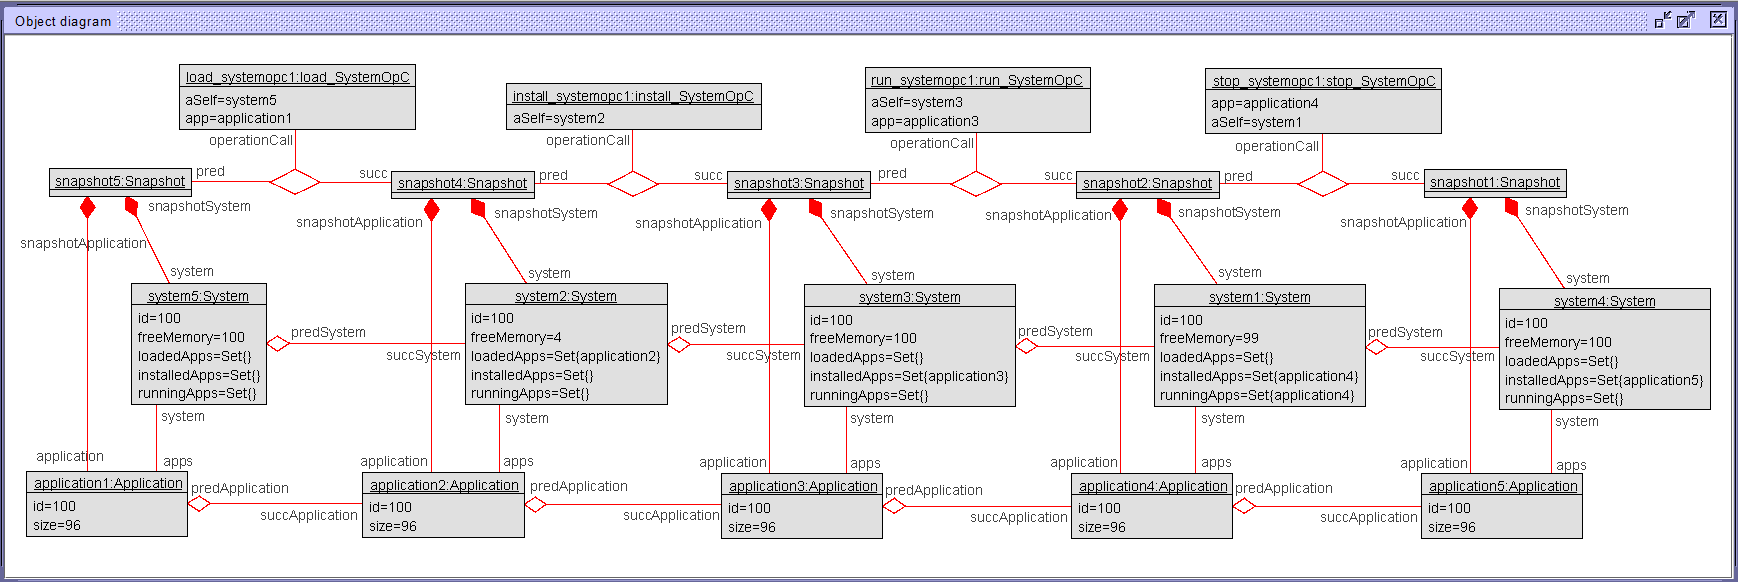
\includegraphics[width=1\textwidth]{figures/c3/CaseStudy_ObjectDiagram.png}
    \caption{A scenario generated by the USE Model Validator.}
    \label{fig:object_diagram_case_study}
\end{figure}

\begin{figure}
    \centering
    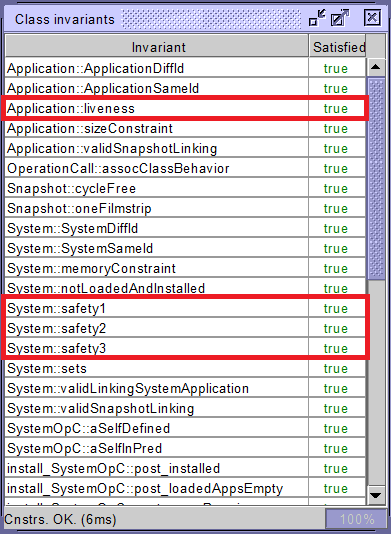
\includegraphics[width=0.4\textwidth]{figures/c3/OCL_result_full_edited.png}
    \caption{OCL result for generated scenario \ref{fig:object_diagram_case_study}.}
    \label{fig:ocl_result_case_study}
\end{figure}
\section{Discussion}

\hspace{1cm} Our TOCL+ approach for specifying and verifying temporal properties in 
UML/OCL models offers several advantages over existing approaches but also comes with 
certain limitations that warrant discussion.

The primary strength of our approach lies in its integration with standard modeling 
environments and tools. By extending OCL rather than introducing an entirely new 
formalism, we maintain compatibility with existing modeling practices while adding 
temporal verification capabilities. This integration allows modelers to work within 
familiar environments while gaining the ability to verify a broader class of 
properties. Our transformation-based approach also offers considerable flexibility. 
By converting TOCL+ specifications to standard OCL constraints on filmstrip models, 
we leverage established OCL tool capabilities without requiring specialized temporal 
verification engines. This provides a pragmatic solution that can be adopted without 
significant infrastructure changes or learning costs. The event-based constructs in 
TOCL+ address a significant gap in existing temporal OCL extensions. While previous 
approaches like TOCL provide temporal operators, they lack robust support for event 
detection and bounded existence properties. Our extensions make it possible to express 
important constraints related to operation calls and state changes, significantly 
broadening the range of verifiable properties.

While effective in practice, our approach has several technical limitations. The OCL 
constraints generated by our transformation can be complex, potentially affecting 
verification performance for large models with numerous temporal properties. These 
constraints involve intricate navigation through snapshots and careful handling of 
object identity, which may impact scalability for very large systems. Our approach 
also requires modelers to add identifier attributes to domain classes to maintain 
object identity across snapshots. This requirement introduces a small burden on 
modelers and slightly modifies the original domain model. A more elegant solution 
would be to handle object identity tracking automatically within the transformation 
framework. The current implementation also has limited support for complex expressions 
within event specifications. For example, nested event expressions or complex guards 
on events might not translate correctly in all cases. This restricts the sophistication 
of temporal properties that can be reliably verified.

From a methodological perspective, our work lacks a formal definition of the TOCL+ 
language and its transformation to OCL. Although our patterns appear to work correctly 
based on empirical evidence from case studies, we haven't provided formal proofs of 
semantic preservation between TOCL+ expressions and their OCL translations. This 
represents a theoretical gap that could affect confidence in the correctness of 
verification results for complex scenarios. Additionally, while our approach handles 
the core temporal operators and event constructs well, it doesn't yet support 
probabilistic or real-time properties. Systems with strict timing requirements or 
probabilistic behavior patterns would require extensions beyond the current 
capabilities.

Several promising research directions emerge from these limitations. The development 
of optimization techniques for the generated OCL constraints could significantly 
improve verification performance. Extending the approach with quantitative time 
constraints would enable verification of real-time properties. Creating a pattern 
library of common temporal verification scenarios with optimized translations would 
make the approach more accessible to practitioners. Enhancing the plugin with more 
intuitive visualizations of counterexamples when temporal properties are violated 
would improve usability. The formal definition of TOCL+ semantics and transformation 
rules, along with mathematical proofs of their correctness, would strengthen the 
theoretical foundations of the approach and provide stronger guarantees about 
verification results.
\section{Summary}
\hspace{1cm} In this chapter, we presented the practical implementation of our TOCL+ 
approach through a plugin for the USE tool and demonstrated its effectiveness through 
a detailed case study. The implementation bridges the gap between the theoretical 
foundations established in Chapter 2 and practical model verification by enabling 
modelers to specify temporal properties in a high-level language while leveraging 
existing OCL verification tools. Our plugin successfully implements the transformation 
rules that convert TOCL+ expressions into equivalent OCL constraints interpreted 
over filmstrip models. The implementation uses ANTLR4 for parsing TOCL+ expressions 
and employs a listener-based approach to systematically translate temporal operators 
and event constructs into structural OCL navigations.

The Software System case study demonstrated how our approach enables verification 
of diverse temporal properties that would be impractical to express in standard OCL. 
The safety properties successfully enforced correct operational sequencing and 
uniqueness constraints, while the liveness property verified eventual progress in 
the system. The complexity of the generated OCL constraints highlights the value of 
our approach: while these constraints involve intricate navigation through snapshots 
and require careful handling of object identity, the TOCL+ specification remains 
simple and intuitive. While our experiments provide empirical evidence supporting 
the correctness of the transformation rules, it's important to note that we have not 
formally proven the correctness of these translations mathematically. Nevertheless, 
the consistent verification results across different temporal properties and scenarios 
provide confidence in the practical applicability of the approach to realistic 
modeling scenarios. The verification performance remained acceptable despite the 
increased complexity of the generated constraints. This chapter thus validates our 
approach experimentally, showing how temporal verification can be effectively integrated 
into standard UML/OCL modeling environments without requiring specialized temporal 
verification tools.
% \hspace{1cm} In this chapter, we presented the practical implementation of our TOCL+ 
% approach through a plugin for the USE tool and demonstrated its effectiveness through 
% a detailed case study. The implementation bridges the gap between the theoretical 
% foundations established in Chapter 2 and practical model verification by enabling 
% modelers to specify temporal properties in a high-level language while leveraging 
% existing OCL verification tools. Our plugin successfully implements the transformation 
% rules that convert TOCL+ expressions into equivalent OCL constraints interpreted 
% over filmstrip models. The implementation uses ANTLR4 for parsing TOCL+ expressions 
% and employs a listener-based approach to systematically translate temporal operators 
% and event constructs into structural OCL navigations.

% The Software System case study demonstrated how our approach enables verification 
% of diverse temporal properties that would be impractical to express in standard OCL. 
% The safety properties successfully enforced correct operational sequencing and 
% uniqueness constraints, while the liveness property verified eventual progress in 
% the system. The complexity of the generated OCL constraints highlights the value of 
% our approach: while these constraints involve intricate navigation through snapshots 
% and require careful handling of object identity, the TOCL+ specification remains 
% simple and intuitive. Our experiments confirm both the correctness of the 
% transformation rules and the practical applicability of the approach to realistic 
% modeling scenarios. The verification performance remained acceptable despite the 
% increased complexity of the generated constraints. This chapter thus validates our 
% approach not just theoretically but in practice, showing how temporal verification 
% can be effectively integrated into standard UML/OCL modeling environments without 
% requiring specialized temporal verification tools.

% 1. Introduction
% Brief overview of the chapter's objectives
% Connection to the theoretical foundation established in Chapter 2
% Outline of what follows in the chapter

% 2. Plugin Implementation
% Architecture and design of the TOCL+ plugin
% Implementation of the TOCL+ parser (generated from ANTLR4 grammar)
% Translation mechanisms for converting TOCL+ to OCL
% Technical details of the id attribute and object identity handling
% Integration with the USE environment

% 3. Software System Case Study
% Detailed description of the Software System model
% Specification of temporal properties using TOCL+
% Step-by-step verification walkthrough
% Results and analysis of verification outcomes
% Demonstration of how various temporal property types are verified

% 4. Summary
% Key findings from the implementation and experiment
% Assessment of the approach's effectiveness
% Implementation challenges and solutions